\documentclass{diploma}

\student{Шадай Дарья Евгеньевна}
\group{М8О-411Б-19}
\theme{Интеграция медицинских справочников в web-приложение onmp.ru}

\supervisor{Пивоваров Дмитрий Евгеньевич}
\firstConsultant{---}
\secondConsultant{---}
\reviewer{---}

\faculty{№ 8 <<Компьютерные науки и прикладная математика>>}
\department{806}
\speciality{02.03.02 <<Фундаментальная информатика и информационные технологии>>}
\profile{Физика}

\departmentFullName{№ 806}
\headOfDepartment{Крылов Сергей Сергеевич}

% Дата. Оставляем пустое место для дня
\date{\uline{\hspace{24pt}} мая \the\year\ года}

\newacronym{api}{API}{Application Programming Interface}
\newacronym{http}{HTTP}{Hypertext Transfer Protocol}
\newacronym{maui}{MAUI}{Multi-platform App UI}
\newacronym{mvvm}{MVVM}{Model-View-ViewModel}
\newacronym{rest}{REST}{Representational State Transfer}
\newglossaryentry{id1}{ % Нужны разные id, можно ставить просто последовательно
    name={Backend},
    description={логика работы сайта, скрытая от пользователя} 
}
\newglossaryentry{id2}{
    name={МКБ},
    description={Международная классификация болезней} 
}
\newglossaryentry{id3}{
    name={$S^{2}$},
    description={формула в списке обозначений} 
}


\addbibresource{main.bib}

% Иллюстрации всегда по центру
\makeatletter
\g@addto@macro\@floatboxreset\centering
\makeatother

\begin{document}
    \maketitle

    % \includepdf[pages=-]{extra/task} % Задание
    \setcounter{page}{2} % Устанавливает счётчик страниц

    \abstract % Структурный элемент: РЕФЕРАТ

 % Реферат

    \tableofcontents % Содержание 
    \termsanddefenitions % Термины и определения
    \listofabbreviations % Перечень сокращений и обозначений
 
    \introduction % Структурный элемент: ВВЕДЕНИЕ

Актуальность данной работы связана с необходимостью оптимизации процесса работы врачей из отделения неотложной медицинской помощи, особенно тех, которые выезжают на вызовы с использованием машин скорой помощи. В настоящее время эти медицинские специалисты заполняют бумажные карты вызова во время осмотра пациента на дому. Однако, такой подход требует ношения с собой больших объемов бумажной документации, что требует больших затрат времени и ресурсов на их заполнение, обработку и хранение.

Переход к электронному заполнению карт вызова имеет ряд значительных преимуществ. Прежде всего, медицинским работникам будет значительно удобнее носить с собой меньшее количество объемной макулатуры, так как электронная форма позволит им быстро и удобно заполнять карты вызова с использованием мобильных устройств, которые они всегда имеют под рукой. Это значительно повысит мобильность и гибкость работы медицинского персонала, позволяя им быстро и эффективно заполнять и обрабатывать данные.

Второе преимущество заключается в возможности хранения электронных карт вызова в интернете. Вместо физического хранения и поиска бумажных документов, медицинские работники смогут сохранять все карты вызова в электронном виде, обеспечивая быстрый и удобный доступ к ним из любого места. Это также позволит легко распечатывать необходимые карты вызова в случае необходимости, например, для передачи другим специалистам или для ведения медицинской документации.

Основной целью данной работы является разработка клиентской части web-сервиса с использованием технологии React.js. Это позволит создать современный и интуитивно понятный пользовательский интерфейс, который облегчит заполнение карт вызова, ускорит процесс ввода данных и повысит эффективность работы медицинских работников.

Был проведен анализ требований к функциональности и пользовательскому интерфейсу web-сервиса, разработана архитектура решения, реализованы необходимые компоненты и проведено тестирование системы. Также была осуществлена интеграция клиентской части с серверной частью системы для обеспечения полной функциональности и взаимодействия с данными.

В рамках данной исследовательской работы можно определить следующие задачи:
\begin{itemize}
    \item Анализ требований к клиентской части web-сервиса: Эта задача включает в себя изучение требований, предъявляемых заказчиком к функциональности и дизайну клиентской части web-сервиса. Необходимо провести тщательный анализ требований, чтобы полноценно понять ожидания и потребности заказчика.
    \item Проектирование клиентской части: Включает разработку детального плана и архитектуры клиентской части web-сервиса. Эта задача включает определение структуры компонентов, взаимодействия между ними, выбор подходящих библиотек и фреймворков для разработки, а также определение способа организации данных и обработки событий.
    \item Разработка функционала авторизации и аутентификации: Данный функционал позволит медицинским работникам входить в систему с использованием уникальных учетных данных. Каждому пользователю будет предоставлен доступ к рабочей среде, где они смогут создавать и использовать собственные шаблоны, а также просматривать и заполнять свои собственные карты вызова.
    \item Создание интерфейса для заполнения и сохранения карт вызова: Разработка пользовательского интерфейса, позволяющего медицинским работникам вводить информацию о состоянии здоровья пациента, тем самым заполняя карту вызова. Данные должны быть легко вводимы и интуитивно понятны, чтобы ускорить процесс заполнения.
    \item Реализация функционала хранения и организации карт вызова в папках: Готовые, Незавершенные, Архив, Шаблоны. Для организации и удобного отображения карт вызова. Это позволит медицинским работникам быстро найти и просмотреть необходимые карты вызова в соответствующих категориях.
    \item Разработка функционала создания и использования шаблонов: Реализация возможности создания шаблонов для быстрого использования частично заполненных карт вызова. Создавая шаблон, пользователь заполняет только некоторые поля карты, чтобы в дальнейшем использовать данный шаблон как основу для карты вызова.
    \item Реализация Функционала поиска, группировки и сортировки карт вызова: Предоставление возможности быстрого поиска нужной информации на основе различных параметров, таких как дата, название карты. Кроме того, группировка и сортировка карт вызова позволят легко ориентироваться в большом объеме данных, что значительно упростит процесс поиска нужной информации.
    \item Тестирование и отладка системы: Проведение тестирования для проверки функциональности и корректности работы системы. Исправление ошибок и устранение неполадок для обеспечения стабильной работы web-сервиса.
\end{itemize}


В данной работе разработка клиентской части web-сервиса осуществляется с использованием React.js - популярной JavaScript-библиотеки для построения пользовательских интерфейсов. React.js предоставляет эффективные инструменты и подходы для создания интерактивных веб-приложений с удобной обработкой данных и переиспользуемыми компонентами. Данная библиотека базируется на концепции компонентного подхода, где пользовательский интерфейс разбивается на независимые компоненты, каждый из которых может иметь свою логику и состояние. Компоненты могут быть переиспользованы, что упрощает разработку и обслуживание приложения.

Дополнительным инструментом к React был выбран Redux. Это библиотека JavaScript, которая предоставляет инструменты для управления состоянием приложения. Она является популярным выбором для разработки сложных и масштабируемых приложений, особенно тех, которые имеют большое количество взаимосвязанных данных.

Redux основывается на концепции однонаправленного потока данных и централизованного хранилища состояния. Вместо того чтобы хранить состояние внутри компонентов, Redux предлагает вынести состояние в отдельное хранилище. Компоненты могут получать доступ к состоянию из хранилища и обновлять его, используя специальные функции.

В целом, совместное использование React и Redux позволяет создавать масштабируемые, предсказуемые и легко поддерживаемые приложения с удобным управлением состоянием \cite{React&Redux}. 

Помимо этого, был выбрана библиотека Axios, которая предоставляет удобный интерфейс для выполнения HTTP-запросов из браузера. Она позволяет взаимодействовать с внешними API, отправлять запросы на сервер и обрабатывать полученные ответы.

Главная цель Axios - упростить и сделать более эффективной работу с HTTP-запросами. Она предоставляет простые методы для отправки различных типов запросов, таких как GET, POST, PUT, DELETE и другие. Кроме того, Axios предоставляет возможности для установки заголовков запроса, обработки ошибок, использования интерсепторов и других функций.

Разработка данного сервиса основывалась на архитектурной методологии Feature-Sliced Design, которая помогает структурировать код и организовать проект на основе функциональных возможностей. Она призвана улучшить масштабируемость, переиспользуемость и поддерживаемость кодовой базы. Основная идея данной методологии заключается в том, что проект разбивается на слои, каждый из которых имеет свою "зону ответственности". Каждый модуль содержит все необходимые компоненты, состояние, стили и логику, связанные с этой функциональностью. Это позволяет разработчикам работать над каждой фичей независимо друг от друга.

Результатом данной работы будет функциональный web-сервис, предоставляющий возможность электронного заполнения и хранения карт вызова для медицинских работников из отделения неотложной помощи. Ожидается, что данное решение значительно улучшит процесс работы медицинских учреждений, сократит временные затраты на бумажную работу и повысит качество медицинской помощи пациентам.

Таким образом, данная дипломная работа имеет практическую значимость и является важным шагом в совершенствовании сферы оказания неотложной медицинской помощи, предлагая инновационное решение, которое отсутствует на рынке.
 % Введение

    \section{ПОСТАНОВКА ЗАДАЧИ}

\subsection{Потребность в улучшении доступности и эффективности медицинской информации}

Современное медицинское обслуживание требует быстрого и удобного доступа к актуальным медицинским справочникам. Однако, в настоящее время, многие справочники представлены в виде бумажных книг или электронных документов, что затрудняет их использование и доступность для медицинского персонала. Для решения этой проблемы необходимо разработать web-справочник, интегрированный с системой отделения неотложной медицинской помощи, который будет упорядочивать и предоставлять все необходимые данные медицинскому персоналу. Такой справочник обеспечит быстрый поиск информации и повысит эффективность работы медицинского персонала.

Однако, следует отметить, что существуют проблемы, которые необходимо решить в процессе разработки и внедрения медицинского справочника в web-приложение отделения неотложной медицинской помощи. Одной из таких проблем является ограниченный доступ к актуальной информации. Традиционные справочники, включая печатные и электронные версии, могут быть устаревшими или не содержать достаточно широкий спектр информации. Это создает трудности при принятии решений в срочных ситуациях и может приводить к задержкам в оказании помощи.

Внедрение медицинского справочника в web-приложение позволит обеспечить медицинскому персоналу быстрый и удобный доступ к актуальным статьям, протоколам, рекомендациям и другой справочной информации. Это улучшит качество медицинской помощи и поможет принимать более обоснованные решения. Важно подчеркнуть, что разработка web-справочника — это не только организация доступа к информации, но и возможность ее постоянного обновления, что позволит всегда иметь актуальные данные и максимально точно оказывать медицинскую помощь.

Другая проблема, которую необходимо решить, связана со временем, затрачиваемым на поиск информации. Врачи скорой помощи часто сталкиваются с необходимостью быстро находить и получать необходимую информацию для оказания срочной помощи. Использование web-приложения с интегрированным справочником значительно сократит время поиска информации и упростит процесс фильтрации и выбора релевантных данных. Благодаря быстрой доступности актуальной информации уменьшаются задержки в предоставлении помощи и улучшаются результаты лечения у пациентов.

Одной из основных сложностей, с которой сталкиваются медицинские работники при поиске информации, является ее поиск и фильтрация по конкретным симптомам, заболеваниям и лекарствам. Различные источники информации могут предоставлять различные данные, что затрудняет их сопоставление и использование. Разработка web-приложения с функцией поиска и фильтрации позволит медицинскому персоналу быстро и точно находить необходимую информацию, основываясь на конкретных параметрах и требованиях. Такой функционал справочника поможет снизить задержки в оказании неотложной медицинской помощи и улучшит точность диагностики и назначения лечения.

Кроме того, недостаточная стандартизация и согласованность информации являются серьезными проблемами в медицине. Различные источники информации могут предоставлять противоречивые и неоднозначные данные, что может привести к путанице и ошибкам в принятии решений. Разработка web-приложения с единым и проверенным источником медицинской информации поможет стандартизировать процедуры и обеспечить согласованность данных, доступных медицинскому персоналу. Это позволит снизить риск возникновения ошибок в диагностике и лечении пациентов.

Важно отметить, что недоступность актуальной и достоверной медицинской информации может повысить риск ошибок и негативных последствий для пациентов. Неправильное применение процедур или назначение неподходящего лечения может иметь серьезные последствия для здоровья и исходов пациентов. Поэтому разработка и внедрение в web-приложения отделения неотложной медицинской помощи медицинского справочника является неотъемлемой частью улучшения качества неотложной медицинской помощи.

Внедрение web-справочника в систему отделения неотложной медицинской помощи поможет оптимизировать и упростить доступ к медицинской информации, что, в свою очередь, позволит значительно повысить качество предоставления медицинской помощи и снизить риск ошибок и задержек в оказании помощи. Кроме того, разработка web-приложения с функцией поиска и фильтрации позволит находить необходимую информацию быстро, точно и на основании конкретных требований. Это является критически важным компонентом для оказания неотложной медицинской помощи и повышения качества медицинской помощи в целом.

\subsection{Анализ существующих подходов к решению проблемы}
В области онлайн-медицинских справочников существует множество ресурсов, которые предлагают информацию о различных заболеваниях, лекарствах, процедурах и других медицинских вопросах. Однако, не все они обладают необходимыми функциональными возможностями и гибкостью настройки, что может затруднять и усложнять поиск и получение нужной информации.

Среди представленных на рынке медицинских справочников можно выделить несколько типов. Один из них - это базовые справочники, которые позволяют осуществлять поиск и просмотр статей, такие как онлайн-ресурсы, медицинские порталы, электронные библиотеки или базы данных. Они обладают широким спектром медицинских материалов, но могут ограничивать пользователей в гибкости настройки и добавления новых материалов.

Другой тип справочников предлагает расширенные функции, такие как фильтрация и сортировка данных, что может быть полезным для быстрого и точного поиска информации. Однако такие решения могут потребовать сложной интеграции и иметь ограниченный доступ к актуальной информации, особенно если они не связаны напрямую с источниками медицинских данных. Кроме того, возможности настройки и добавления новых материалов также могут быть ограничены.

Несмотря на некоторые недостатки, медицинские справочники имеют важные преимущества, такие как доступ к актуальной медицинской информации, удобство использования и возможность получения справочных данных в любое время. Однако, некоторые из них могут иметь недостатки, такие как ограниченный объем информации, отсутствие персонализации, невозможность обновления данных в реальном времени и ограниченный доступ к некоторым функциям без платной подписки.

В рамках проекта мы сосредоточимся на создании микросервиса, реализующего функции справочника, для web-приложения по электронному заполнению медицинских карт, который преодолевает эти недостатки. Приложение будет обеспечивать быстрый доступ к информации о заболеваниях и их симптомах, соблюдая актуальные медицинские стандарты, а также предлагать удобный интерфейс и быстрый доступ к данным. Оно также будет обладать гибкостью настройки и возможностью обновления данных, чтобы обеспечить врачам всегда актуальную информацию. Все это позволит сделать приложение максимально полезным и удобным для пользователей.

Web-приложения медицинских справочников могут варьироваться по функционалу и целям. Рассмотрим некоторые из них:
\begin{itemize}
    \item основные медицинские справочники: этот тип справочника предоставляет общую медицинскую информацию, включая симптомы, диагнозы, лечение и рекомендации. Он может включать информацию о различных заболеваниях, медицинских процедурах, лекарственных препаратах и т.д. Такой справочник позволяет врачам быстро получить доступ к основным медицинским знаниям и руководствам. Недостатком таких справочников является то, что они могут быть слишком общими и не всегда содержать достаточно деталей или актуальной информации для специфических случаев или редких заболеваний. Важно обеспечить актуализацию и достоверность информации, чтобы предотвратить ошибки в диагностике или лечении;
    \item экстренные справочники: эти справочники ориентированы на оказание первой помощи и управление экстренными ситуациями. Они содержат информацию о действиях, необходимых в случае серьезных травм, сердечного приступа, инсульта и других критических состояниях. Такие справочники могут включать шаг за шагом инструкции, видеоуроки и иллюстрации, чтобы помочь врачам и работникам скорой помощи принять быстрые и правильные решения. Такие справочники ограничены тем, что некоторые ситуации могут требовать индивидуального подхода и консультации с медицинскими специалистами;
    \item фармакологические справочники: этот тип справочника содержит информацию о лекарственных препаратах, включая их названия, дозировки, побочные эффекты, противопоказания и инструкции по применению. Такие справочники помогают врачам подобрать правильные лекарства для конкретных пациентов и обеспечивают информацию о взаимодействии препаратов и других особенностях. Такие справочники ограничены тем, что принятие решений о лечении требует оценки индивидуальных особенностей пациента и консультации с медицинскими специалистами;
    \item справочники по специализированным областям: такие справочники посвящены конкретным специализированным областям медицины, таким как педиатрия, гинекология, кардиология, онкология и другие. Они содержат специфическую информацию, связанную с данной областью медицины, и могут быть полезными для специалистов, работающих в этих областях.
\end{itemize}

После консультации с врачом, работающим в отделении неотложной медицинской помощи, было принято решение о создании справочника, включающегося в список общих медицинских справочников. Целью данного справочника является обеспечение быстрого доступа к информации о болезнях и их симптомах, чтобы облегчить и ускорить процесс диагностики в рамках работы скорой помощи, с учетом последних медицинских стандартов. Для достижения этой цели, приложение должно быть удобным в использовании и обеспечивать быстрый доступ к данным, чтобы обеспечить эффективность и оперативность в работе. Важно также обеспечить постоянное обновление и актуализацию информации, чтобы врачи всегда имели доступ к последним рекомендациям и протоколам.

При реализации проекта, интегрированный в web-приложение медицинский справочник получит преимущества перед уже существующими решениями, так как он будет иметь возможность интеграции с текущим приложением для электронного оформления медицинских карт. Это означает, что врачи смогут использовать справочник непосредственно в процессе работы с пациентами, без необходимости переключаться между разными системами. 

\subsection{Обоснование цели и задач, техническое задание на разработку}
В настоящее время врачи скорой помощи работают в условиях, требующих оперативности и своевременных решений. Для того чтобы быстро получить необходимую информацию, им необходим быстрый доступ к актуальной информации, которая должна быть доступна на различных устройствах, включая смартфоны и планшеты. Кроме того, учитывая динамическую природу работы врачей скорой помощи, важно, чтобы справочник был легко доступен и имел интуитивно понятный интерфейс.

Разработка справочника, интегрированного в web-приложение для заполнения медицинских карт, позволит врачам скорой помощи получать быстрый доступ к необходимой информации, что позволит оптимизировать процесс оказания медицинской помощи, ускорить принятие решений и повысить качество обслуживания пациентов. Однако, для того чтобы реализовать эту идею, необходимо учитывать множество требований, таких как фильтрация и группировка информации, удобный интерфейс и т.д.

Поэтому целью данной работы является внедрение медицинских справочников в web-приложение отделения неотложной медицинской помощи с учетом всех вышеперечисленных требований. Такой подход позволит медицинскому персоналу быстро находить необходимую информацию, что повысит их эффективность и улучшит качество обслуживания пациентов.

Для реализации цели работы были поставлены следующие задачи:
\begin{itemize}
    \item подготовка тестовых данных;
    \item разработка макета web-страницы;
    \item разработка каркаса web-справочника в соответствии с макетом с основными функциональными компонентами, такими как поисковая строка, категоризация статей;
    \item реализация функций добавления, редактирования и удаления статей справочника;
    \item настройка взаимодействия между web-приложением и удаленным web-сервером, обеспечивающее передачу и получение данных.
\end{itemize}

Также web-приложение должно иметь интуитивно понятный интерфейс, который обеспечит удобный поиск, фильтрацию и просмотр информации. Web-приложение должно быть интегрировано в существующую систему электронного оформления медицинских карт, чтобы врачи могли получать доступ к справочной информации без необходимости переключения между различными приложениями.

По завершении проекта, ожидается, что врачи скорой помощи смогут быстро получать доступ к актуальной и проверенной медицинской информации. Более того, интеграция существующего приложения для электронного оформления медицинских карт позволит оптимизировать процесс оказания медицинской помощи, значительно упростить процесс работы и повысить эффективность обслуживания пациентов в отделении неотложной медицинской помощи. % Основная часть
    \section{РАЗРАБОТАННОЕ РЕШЕНИЕ}

\subsection{Подход к решению задачи}

После консультации с врачом, работающим в отделении неотложной медицинской помощи, были выделены следующие критерии для эффективного решения задачи отображения страниц справочника:

\begin{itemize}
    \item интерфейс: основной принцип разработки интерфейса состоит в его интуитивной понятности, чтобы пользователи могли легко ориентироваться на страницах справочника. Все элементы управления должны быть расположены таким образом, чтобы их использование было интуитивно понятным и не требовало больших усилий;
    \item оптимизация информации: учитывая условия работы в отделении неотложной медицинской помощи, статьи справочника должны быть оптимизированы с точки зрения предоставления только самой важной и необходимой информации. Отсеивание избыточных данных и акцентирование внимания на ключевых сведениях позволит медицинскому персоналу быстро получать нужную информацию без необходимости тратить время на чтение больших объемов текста;
    \item группировка и функция поиска: для удобства навигации и быстрого доступа к нужным сведениям, статьи в справочнике должны быть сгруппированы по соответствующим категориям или темам. Также необходимо реализовать эффективную функцию поиска, которая позволит пользователям быстро находить нужные статьи. Поисковой механизм должен быть точным и эффективным, чтобы облегчить работу медицинского персонала в условиях неотложной помощи;
    \item функция добавления статей: для обеспечения актуальности и расширения информационной базы справочника, необходима возможность добавления новых статей. Эта функция должна предоставлять пользователю удобный интерфейс, где можно будет ввести заголовок, категорию, и внести основной текст статьи. Эта функция должна быть доступна только пользователям с соответствующими правами доступа;
    \item функция редактирования статей: для обновления информации в справочнике, пользователи с соответствующими правами доступа должны иметь возможность редактировать уже существующие статьи. Она позволит вносить изменения в текст статьи, обновлять связанные атрибуты (например, категорию или определение) и улучшать содержание для точности и актуальности данных. Интерфейс редактирования должен быть интуитивно понятным, позволяя пользователям легко найти и внести необходимые изменения в статьи;
    \item функция удаления статей: для поддержания надежности и актуальности информации в справочнике, необходимо предусмотреть функцию удаления статей, которая была бы доступна пользователям с соответствующими правами доступа. Также необходимо добавить подтверждение действия перед окончательным удалением статьи, чтобы пользователи могли избежать нежелательных ошибок;
    \item открытие страниц в новых вкладках: для обеспечения быстрого возврата к предыдущей открытой статье, страницы справочника должны открываться в новых вкладках браузера. Это позволит врачам легко переключаться между статьями, сохраняя контекст работы и экономя время на поиске и повторном открытии страниц.
\end{itemize}

Учитывая эти требования, при разработке интерфейса отображения страниц справочника необходимо обеспечить простоту использования, логичную структуру, адаптивность к различным устройствам и возможность интеграции с дополнительными функциональностями для облегчения работы пользователей и обеспечения удобства использования сервиса.

Алгоритм работы web-справочника включает следующие шаги:

\begin{itemize}
    \item осуществляется запрос на сервер, по которому происходит извлечение данных о заголовках и категориях статей из базы данных;
    \item по полученным данным все статьи группируются по категориям;   
    \item пользователь взаимодействует с интерфейсом web-справочника, вводя запросы в поисковую строку или выбирая категории и просматривая статьи из списка;
    \item введенные запросы и выбранные параметры передаются в соответствующие функции, которые обрабатывает запросы и выполняет соответствующие действия;
    \item программа осуществляет поиск данных, используя предопределенные алгоритмы поиска и фильтрации;
    \item при клике на заголовок статьи осуществляется запрос на сервер, по которому происходит извлечение данных о выбранной статье;
    \item полученные данные отображаются пользователю в удобном и понятном виде.
\end{itemize}

\subsection{Обоснование стека используемых технологий}

JavaScript является одним из самых популярных языков программирования, используемых для разработки web-приложений. Он является клиентским языком программирования, выполняющимся в браузере пользователя и позволяющим добавлять динамическое поведение к web-страницам. JavaScript обеспечивает множество возможностей для создания интерактивных и отзывчивых пользовательских интерфейсов \cite{JavaScript}.

JavaScript также обладает множеством других возможностей, которые делают его привлекательным для разработки web-приложений. Он поддерживает асинхронное программирование, что позволяет выполнять задачи без блокирования основного потока выполнения. JavaScript имеет множество встроенных функций и методов, которые упрощают манипуляцию с DOM (Document Object Model), обработку событий, отправку HTTP-запросов и многое другое.

В целом, JavaScript является мощным инструментом для разработки веб-приложений. С его помощью разработчики могут создавать интерактивные пользовательские интерфейсы, обрабатывать данные, взаимодействовать с сервером и использовать различные фреймворки и библиотеки, такие как React и Angular, для создания масштабируемых и производительных приложений.

При разработке клиентской части web-приложения выбор стоял между двумя фреймворками — React и Angular. Рассмотрим их подробнее:

React — это библиотека для разработки пользовательских интерфейсов, фокусирующаяся на создании компонентов. Он предоставляет мощные инструменты для управления состоянием и эффективного рендеринга обновлений. React использует JSX для объединения JavaScript и HTML-подобного синтаксиса \cite{React}.

Angular — это полноценный фреймворк для разработки web-приложений. Он предоставляет инструменты для создания компонентов, управления состоянием, маршрутизации, обработки событий и многое другое. Angular использует TypeScript и шаблоны HTML для создания приложений \cite{Angular}.

Сравним их:

\begin{itemize}
    \item размер и сложность: React является более легковесным и простым в освоении по сравнению с Angular. Angular имеет больший размер и более сложную структуру, что может потребовать больше времени для изучения и освоения;
    \item гибкость и расширяемость: React предоставляет большую гибкость и свободу в выборе других инструментов и библиотек, таких как маршрутизация или управление состоянием (Redux, MobX и другие). Angular предлагает широкий набор инструментов встроенно, что упрощает разработку приложений, но может быть менее гибким при необходимости использования сторонних решений;
    \item производительность: оба фреймворка обеспечивают хорошую производительность, но React, благодаря своему виртуальному DOM и механизму сравнения изменений, может быть более эффективным в обновлении компонентов.
\end{itemize}

Проанализировав преимущества и недостатки каждого фреймворка, выбор пал на React. В обоснование этого выбора следует отметить несколько причин:

\begin{itemize}
    \item легкость освоения и использования: React предоставляет простой и интуитивно понятный подход к разработке пользовательских интерфейсов. Его основной концепцией является создание компонентов, что позволяет разбить интерфейс на небольшие независимые блоки. Это упрощает понимание и модификацию кода, а также облегчает внедрение новых разработчиков в проект;
    \item эффективный рендеринг обновлений: React использует виртуальный DOM и механизм сравнения изменений, что позволяет эффективно обновлять только необходимые части интерфейса при изменении состояния. Это особенно полезно в условиях работы веб-справочника, где быстрое обновление данных и реакция на взаимодействие пользователя являются важными требованиями;
    \item обширная экосистема и сообщество: React имеет огромную экосистему, включающую библиотеки и инструменты для различных задач разработки, такие как маршрутизация, управление состоянием и тестирование. Это позволяет выбирать наиболее подходящие инструменты и расширения для вашего проекта. Кроме того, React обладает активным и развитым сообществом разработчиков, где можно получить поддержку, решить проблемы и узнать о лучших практиках;
    \item популярность и поддержка: React является одним из самых популярных инструментов для разработки пользовательских интерфейсов. Благодаря своей популярности, React имеет широкую поддержку и активное развитие. Это обеспечивает стабильность, надежность и постоянное обновление библиотеки.
\end{itemize}

Для взаимодействия приложения с сервером был выбран REST API (Representational State Transfer Application Programming Interface) — это архитектурный стиль для разработки web-сервисов. REST API предоставляет набор принципов, которые определяют, как взаимодействовать с web-сервисом. Он использует стандартные HTTP-методы, включая GET, POST и DELETE, для выполнения операций над ресурсами. REST API обеспечивает гибкость и масштабируемость взаимодействия между клиентом и сервером, позволяя выполнять различные операции, такие как создание, чтение, обновление и удаление данных \cite{API}.

При проектировании и разработке web-приложений, использование API-запросов, таких как GET- и POST-запросы, имеет несколько преимуществ:
\begin{itemize}
    \item получение данных с сервера: использование GET-запросов позволяет получать данные с сервера, необходимые для работы и отображения в приложении. Это может быть информация о пользователях, продуктах, новостях или любых других данных, которые приложение должно получать извне. POST-запросы, в свою очередь, используются для отправки данных на сервер, например, при создании новых записей или отправке форм;
    \item асинхронность и отзывчивость: и GET-запросы, и POST-запросы выполняются асинхронно, что позволяет приложению продолжать работу, пока данные отправляются или обрабатываются на сервере. Это поддерживает отзывчивый пользовательский интерфейс и позволяет пользователям взаимодействовать с приложением без задержек;
    \item обновление данных: POST-запросы часто используются для обновления данных на сервере. Например, при редактировании информации о пользователе или изменении статуса заказа. Отправка POST-запроса с обновленными данными позволяет приложению синхронизироваться с сервером и обновить информацию;
    \item удобство и простота использования: GET- и POST-запросы являются одними из наиболее распространенных типов запросов и относительно легко реализуются в коде приложения. Для выполнения запросов на сервер существуют различные библиотеки и инструменты, такие как Fetch API или axios, которые упрощают отправку запросов и обработку полученных данных;
    \item кэширование: и GET-запросы, и POST-запросы могут использовать кэширование для оптимизации производительности. Однако обычно POST-запросы не кэшируются, поскольку они могут иметь побочные эффекты на сервере, такие как изменение данных.
\end{itemize}

Также была выбрана библиотека компонентов для React — MUI \cite{MUI}. Она предоставляет готовые стилизованные компоненты, которые соответствуют принципам Material Design. Использование MUI упростит разработку, добавление стилей и создание современного и эстетически привлекательного интерфейса.  Библиотека MUI предлагает широкий набор компонентов, таких как кнопки, формы, таблицы, диалоги, навигационные панели и многое другое. Каждый компонент разработан с учетом принципов Material Design, что обеспечивает современный и согласованный внешний вид пользовательского интерфейса.

Одной из ключевых особенностей MUI является ее гибкость и настраиваемость. Компоненты MUI могут быть легко настроены и адаптированы под конкретные требования проекта. Они также поддерживают темизацию, что позволяет изменять внешний вид компонентов, чтобы они соответствовали дизайну проекта.

MUI обладает активным сообществом разработчиков и постоянно обновляется, предоставляя новые компоненты и функциональность. Она также интегрируется с другими популярными инструментами и библиотеками, такими как React Router и Redux, что делает ее идеальным выбором для разработки современных web-приложений на базе React.

Для создания макета было выбрано web-приложение Figma \cite{Figma}. Figma - это web-приложение для дизайна интерфейсов, которое позволяет дизайнерам и командам работать над созданием и прототипированием пользовательских интерфейсов. Figma предоставляет инструменты для создания макетов, иллюстраций, прототипов и совместной работы над проектами в режиме реального времени.

Основная особенность Figma заключается в его возможности работать на разных платформах и быть доступным через web-браузер без необходимости установки дополнительного программного обеспечения. Это позволяет дизайнерам и командам с легкостью сотрудничать над проектами, делиться макетами и получать обратную связь в режиме реального времени.

Также Figma обладает широким набором инструментов для создания и редактирования дизайна, включая возможность работы с векторной графикой, добавления интерактивных элементов и создания анимаций. Он также предлагает функции комментирования и обсуждения, что упрощает процесс сотрудничества и согласования изменений в проекте.

Все это позволяет создать современный и интуитивно понятный интерфейс, что особенно важно для удобства использования web-справочника.

\subsection{Описание программной разработки}

В рамках программной разработки функционального web-справочника в приложении электронного заполнения медицинских карт было выполнено несколько шагов.

Сначала был разработан макет. С помощью инструмента Figma был создан макет будущей страницы справочника, представленный на рисунке~\ref{fig:page-model}, на котором расположены все необходимые элементы, такие как статьи, разделенные по категориям, и поисковая строка.

\begin{figure}
  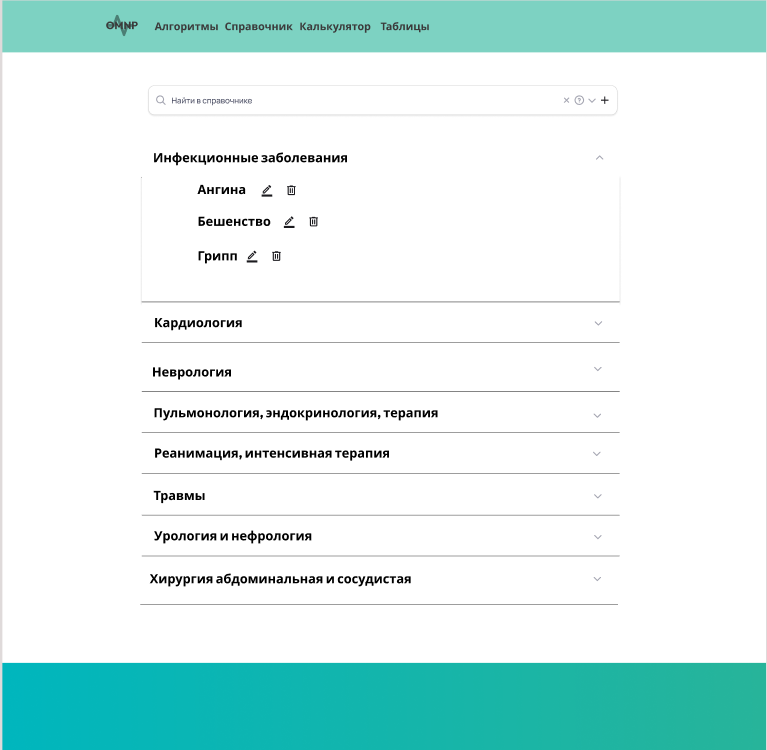
\includegraphics[scale=0.5]{styles/diploma/inc/Макет.png}
  \caption{Макет страницы справочника}
  \label{fig:page-model}
\end{figure}

Затем была проведена подготовка справочных данных. Консультирующий врач предоставил распечатанные примеры справочных материалов, представленные на рисунке~\ref{fig:ex-ref}, которые были использованы для составления информации о болезнях в формате определения, инкубационного периода (если есть), симптомов, форм заболевания (если есть). Дополнительно, информация была взята с сайтов <<Медицинская энциклопедия>>\cite{Encyclopedia}, <<Справочник MSD>>\cite{MSD} и телеграм-бота <<PARAMEDIC (шпаргалки)>>\cite{Paramedic}. Все справочные данные проверены и подтверждены консультирующим врачом.

\begin{figure}
  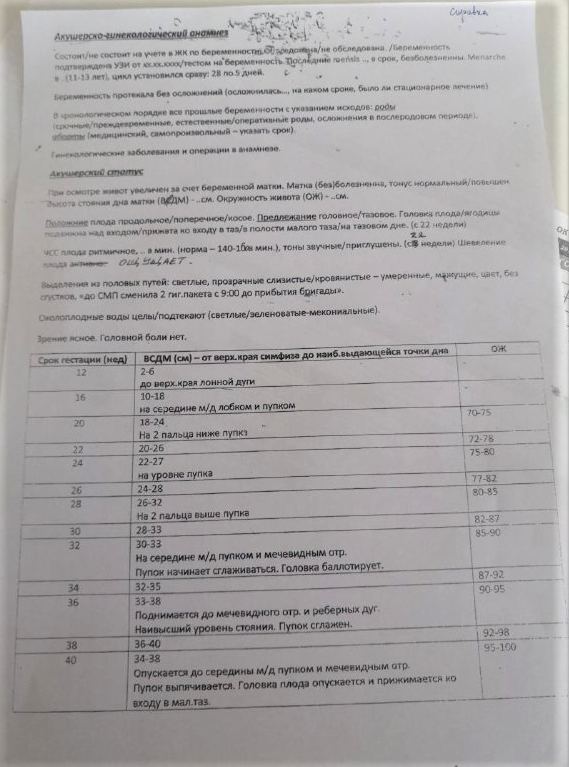
\includegraphics[scale=0.5]{styles/diploma/inc/ex-ref.png}
  \caption{Пример распечатанного справочного материала}
  \label{fig:ex-ref}
\end{figure}

Для полной реализации проекта и разработки функционала, был создан проект на платформе GitLab, включающий все необходимые компоненты для электронного заполнения медицинских карт. Основная разработка функционала справочника происходила в папке <<src/pages/feature-pages/dictionary>>.

В рамках разработки был создан компонент ArticleModel.jsx, который содержит функцию createArticleData. Эта функция принимает заголовок статьи и данные из API-ответа и возвращает структурированные данные о статье, которые затем используются для ее отображения на странице.

На следующем рисунке~\ref{src:src2} показан листинг, который содержит функцию createArticleData:

 \begin{figure}
 \begin{lstlisting}[language=Python]
export const createArticleData = (title, data) => {
    const { tag, description, symptomps, period, forms } = data[title];
    const formDescriptions = data[title]['form descriptions'];
    const formSymptoms = data[title]['form symptomps'];
  
    return {
      tag,
      title,
      description,
      symptomps,
      period,
      forms,
      formDescriptions,
      formSymptoms,
    };
  };
\end{lstlisting}
\caption{Функция createArticleData}
\label{src:src2}
\end{figure}

Затем был создан компонент ArticlePage.jsx, который отображает текст статьи. При загрузке страницы, с помощью хука useEffect, происходит получение данных статьи из sessionStorage. Если данные уже были сохранены, то они отображаются на странице. В противном случае выводится сообщение о том, что статья не найдена.

На главной странице справочника присутствует поиск по названию статьи, кнопка добавления новой статьи и аккордеон, заголовками которого выступают категории, а содержимым являются статьи, соответствующие этим категориям. У каждой статьи находятся кнопки редактирования и удаления. Эти функции были реализованы с использованием компонентов MUI (Material-UI). При изменении значения поиска происходит фильтрация статей и категорий. Также присутствует возможность сворачивания/разворачивания всех категорий с помощью кнопки. При клике на статью происходит открытие новой вкладки с полной статьей или перенаправление на страницу <<Статья не найдена>>, если статья отсутствует.

Для обеспечения адресации страниц справочника использовался React Router: была реализована маршрутизация и подключены компоненты для каждой страницы, включая страницу справочника.

После завершения разработки интерфейса в соответствии с макетом, был добавлен файл mockData.json, содержащий пример данных, которые будут передаваться с сервера. После тестирования приложения с этими данными, была настроена связь web-приложения с удаленным сервером с использованием REST API. В моем проекте для получения медицинских данных с сервера необходимо использовать GET-запрос. При загрузке приложения, с помощью функции useEffect, происходит отправка асинхронного запроса POST на адрес <<http://188.225.78.148/api/v1/>>. В заголовке запроса также передается токен CSRF для авторизации. Полученные данные в формате JSON обрабатываются и структурируются с использованием функции createArticleData. Эта функция принимает заголовок статьи и данные из API-ответа, а затем извлекает необходимую информацию, такую как категория, описание, симптомы, период, формы и т.д. Сначала мы используем GET-запрос для получения информации обо всех парах "заголовок статьи":"категория", которые есть на сервере. С помощью этих данных мы формируем аккордеоны. Когда пользователь нажимает на заголовок статьи, эта статья открывается в новой вкладке. Затем используется второй GET-запрос, в который передается заголовок статьи. На выходе мы получаем объект articleData, который содержит структурированную информацию о выбранной статье. Затем мы выводим эту информацию на странице.

Для добавления новой статьи используется POST-запрос, в который передаются параметры <<name>> (название заболевания), <<tag>> (категория заболевания), <<description>> (описание заболевания), <<period>> (продолжительность болезни или ее инкубационный период), <<symptoms>> (симптомы заболевания), <<forms>> (формы заболевания), <<forms descriptions>> (описания форм заболевания), <<forms symptomps>> (симптомы форм заболевания). Параметры <<name>> и <<tag>> не могут быть пустыми. Для удаления статьи используется метод DELETE, в который передается название статьи. Для редактирования статьи, используется форма, содержащая такие же параметры, как при добавлении новой статьи. При нажатии на кнопку <<Сохранить>>, если поля <<name>> и <<tag>> не пустые, происходит запрос DELETE, в который передается название статьи, которую редактировали, а затем происходит POST-запрос, в который передаются параметры, переданные в форме редактирования статьи. Если хотя бы одно из полей <<tag>> или <<name>> пустое, то форма запретит сохранение такой статьи.

Такая интеграция с удаленным сервером через REST API позволяет приложению получать актуальные медицинские данные и обновлять базу данных в соответствии с внесенными изменениями. Это обеспечивает актуальность и достоверность информации в web-справочнике, а также позволяет медицинским работникам скорой помощи оперативно получать необходимую информацию для принятия решений.

В результате программной разработки был создан функциональный web-справочник в приложении для электронного заполнения медицинских карт. Этот справочник предоставляет возможность пользователям осуществлять поиск и отображение медицинской информации, а также функции по добавлению, редактированию и удалению статей, значительно упрощая процесс заполнения медицинских карт и обеспечивая доступ к необходимым справочным материалам.

    \section{РЕЗУЛЬТАТЫ РАБОТЫ}

\subsection{Характеристика условий и места применения разработки}

Web-справочник был специально разработан для использования медицинскими работниками скорой медицинской помощи в условиях их оперативной деятельности. Из-за особенностей этой области и ее требований, разработанный справочник обеспечивает оптимальную поддержку и удобство использования в рабочих условиях, связанных с оказанием скорой медицинской помощи. Он предоставляет удобный и мгновенный доступ к необходимой медицинской информации, что позволяет работникам быстро находить нужные данные и принимать информированные решения.

Web-справочник находит свое применение в следующих ситуациях:

\begin{itemize}
    \item экстренные ситуации: в случаях, требующих немедленной реакции, медицинским работникам необходимо быстро получить доступ к актуальной информации о симптомах, диагнозах и процедурах оказания помощи. Web-справочник обеспечивает оперативный поиск и доступ к рекомендациям и протоколам, помогая медицинским работникам принимать правильные решения в экстренных ситуациях;
    \item полевые условия: врачи и санитары, работающие на местах происшествий или в других условиях, где доступ к стационарным справочникам ограничен, могут полагаться на web-справочник для получения необходимой информации о болезнях;
    \item обновление знаний: web-справочник предоставляет возможность медицинским работникам быть в курсе последних достижений в медицинской науке и практике. Для обновления знаний, материалы в справочнике могут быть обновлены администратором или пользователями с соответствующими правами доступа. Таким образом, медицинские работники могут легко получать информацию из обновленных источников и оставаться информированными о последних достижениях в своей области.
\end{itemize}

Важными характеристиками использования разработанного web-справочника в работе медицинских работников скорой помощи являются:

\begin{itemize}
    \item оптимизированный поиск информации: медицинским работникам скорой помощи часто требуется мгновенный доступ к конкретным медицинским справочным данным. Разработанный справочник обеспечивает быстрый и эффективный поиск по ключевым статьям, позволяя оперативно находить нужную информацию и принимать соответствующие решения;
    \item удобное хранение данных: разработанный справочник хранит данные по категориям, что дает медицинским работникам скорой помощи быстрый доступ к наиболее важным и актуальным данным, если у них нет времени выполнять поиск;
    \item обновляемая и достоверная информация: в медицинской практике необходимо иметь доступ к актуальным и проверенным справочным материалам. Разработанный справочник может обновляться и поддерживаться, обеспечивая медицинским работникам достоверную информацию, соответствующую последним стандартам и протоколам лечения;
    \item добавление, редактирование и удаление статей: дополнительно, в справочнике можно добавлять, редактировать и удалять статьи. Эта функциональность позволяет пользователям активно участвовать в обновлении и сопровождении содержимого справочника, адаптировать его под новые требования и предоставлять актуальную информацию. Пользователи могут вносить изменения, исправлять неточности, добавлять новые материалы или удалять устаревшие записи, обеспечивая таким образом достоверность и актуальность данных в справочнике. Это дает медицинскому персоналу скорой помощи возможность влиять на содержание справочника и обеспечивает динамическую и адаптивную природу данного ресурса;
    \item возможность расширенного поиска: web-справочник также предоставляет удобную функцию перехода на посторонний сайт для дополнительного поиска информации. При использовании поисковой строки в справочнике, пользователю отображается опция <<Поиск по справочнику MSD>> с прикрепленной ссылкой. При клике на эту ссылку, пользователь может открыть страницу с результатами поиска по своему запросу на постороннем сайте в новой вкладке браузера. Таким образом, врачам не требуется открывать другой сайт или повторно вводить запрос, сохраняя все процессы поиска и получения информации в одном месте — в web-справочнике. Это обеспечивает удобство использования и экономит время медицинского персонала.
\end{itemize}

При тестировании web-справочника были проведены проверки, направленные на обеспечение корректности, надежности и эффективности приложения. Главной целью тестирования было проверить соответствие разработанного функционала заявленным требованиям.

Одним из аспектов, проверенных в ходе тестирования, было отображение и доступность информации в интерфейсе web-справочника. Важно было убедиться, что информация корректно отображается пользователю и соответствует заданному макету. Это позволяет обеспечить удобство использования приложения и удовлетворение потребностей пользователей.

Другим аспектом тестирования была проверка правильности функционирования различных модулей и компонентов приложения. В ходе тестирования проверялась правильность работы функции поиска по названию статьи. 

Результаты тестирования подтверждают соответствие разработанного приложения заявленным требованиям, данные функциональности работают корректно и обеспечивают надежность и эффективность его работы.

\subsection{Результаты работы разработанного программного кода}

В результате работы был создан web-справочник, который предоставляет пользователю следующие функциональности:

\begin{itemize}
    \item интуитивно понятный интерфейс пользователя: интерфейс, показанный на рисунке~\ref{fig:main-page}, разработан с учетом простоты и интуитивности, чтобы пользователи могли быстро ориентироваться и находить нужную информацию. Он предоставляет удобную навигацию, плавные переходы между разделами, интуитивные иконки и элементы управления, а также четкую организацию контента;

\begin{figure}
  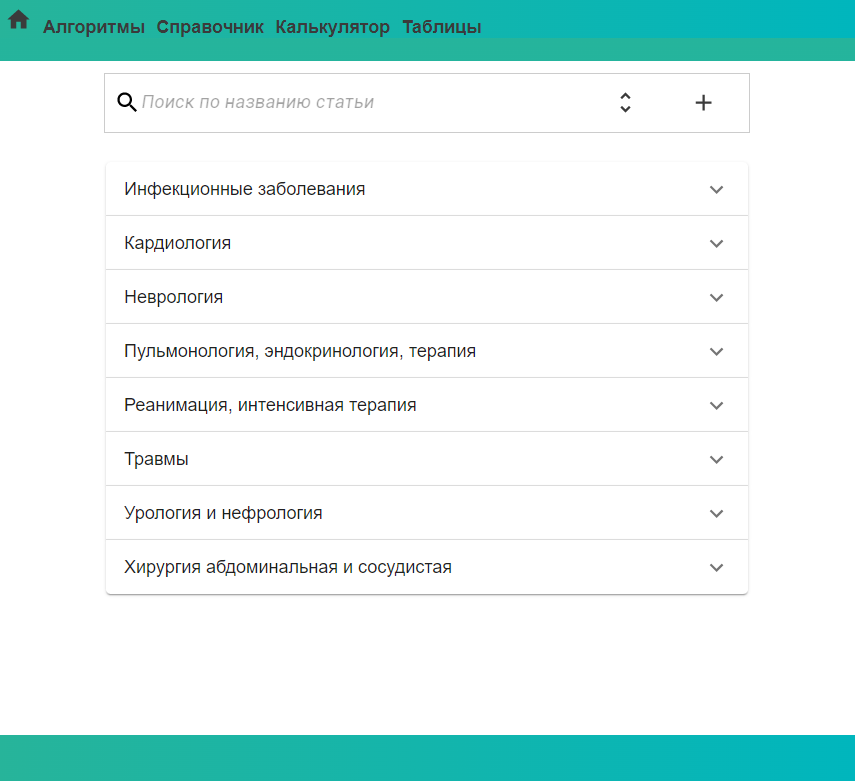
\includegraphics[scale=0.6]{styles/diploma/inc/ГлСтраница.png}
  \caption{Интерфейс справочника}
  \label{fig:main-page}
\end{figure}

    \item поисковая строка: в справочнике реализована поисковая строка, представленная на рисунке~\ref{fig:search}, которая позволяет пользователям вводить ключевые слова и получать соответствующие результаты поиска. Механизм поиска анализирует запросы пользователей и находит наиболее релевантные статьи и информацию, соответствующую введенным ключевым словам;

\begin{figure}
  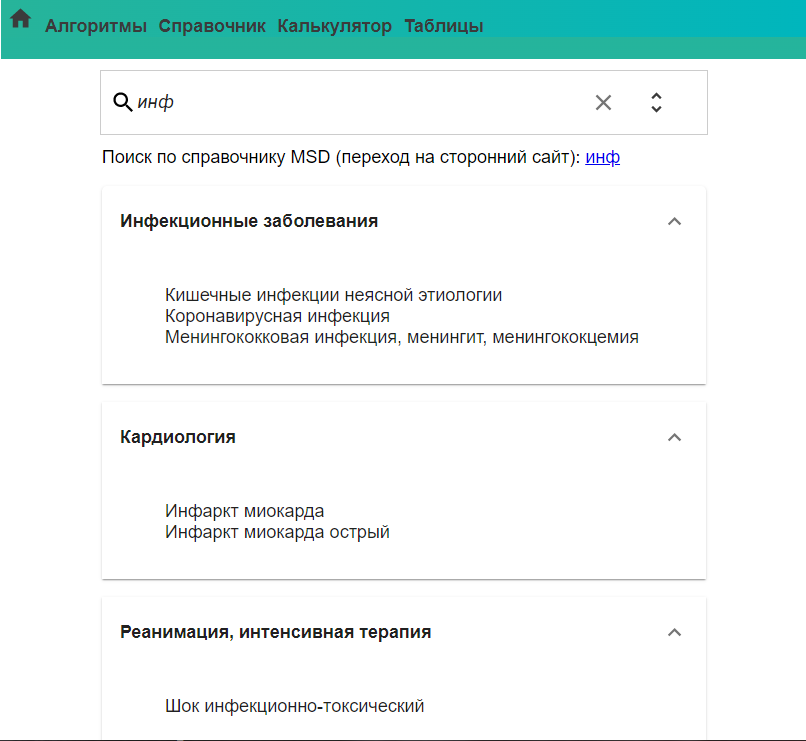
\includegraphics[scale=0.6]{styles/diploma/inc/Поиск.png}
  \caption{Поиск по справочнику}
  \label{fig:search}
\end{figure}

    \item категории для классификации информации: справочник предоставляет организацию информации в виде категорий, что облегчает пользователю поиск нужных разделов. Пользователи могут выбирать соответствующую категорию и легко получать доступ к нужным статьям внутри этой категории;
    \item отображение информации: разработанный справочник отображает информацию, содержащуюся в статье, соответствующим образом, согласно шаблону, указанному в предыдущих разделах. После выполнения поиска или выбора статьи пользователь может просмотреть кликнуть на статью. Если содержимое статьи есть в базе данных, открывается страница с текстом статьи, как на рисунке~\ref{fig:article}. В случае, если текст статьи не загружен в справочник, происходит переадресация на соответствующую страницу;

\begin{figure}
  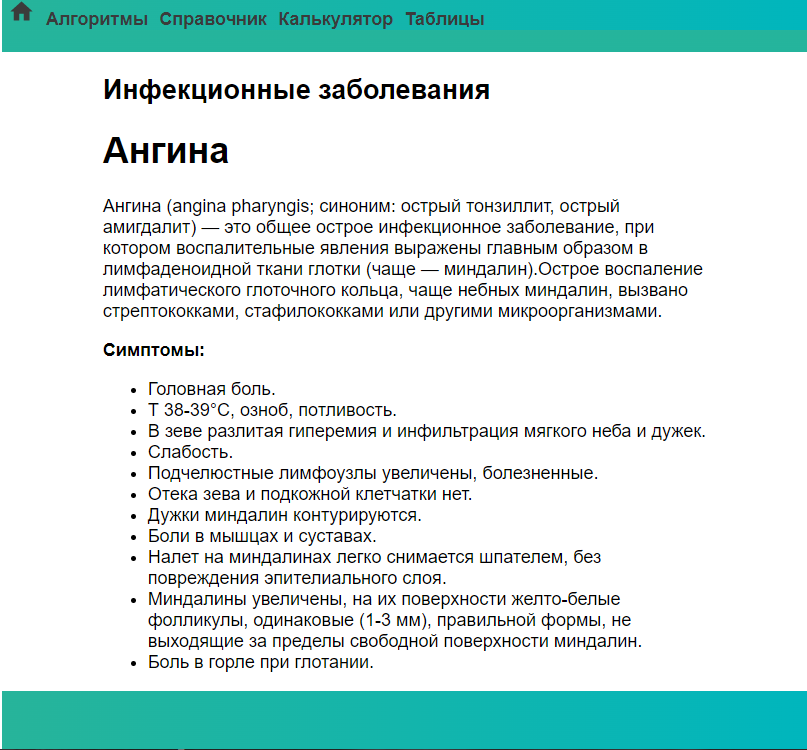
\includegraphics[scale=0.6]{styles/diploma/inc/Статья.png}
  \caption{Отображение статьи справочника}
  \label{fig:article}
\end{figure}

    \item функция добавления статей: администраторы и авторизованные пользователи с правами редактирования имеют возможность добавлять новые статьи в справочник. При добавлении статьи необходимо заполнить соответствующие поля, представленные на рисунке~\ref{fig:add}. После сохранения, новая статья становится доступной для просмотра и поиска в справочнике;

\begin{figure}
  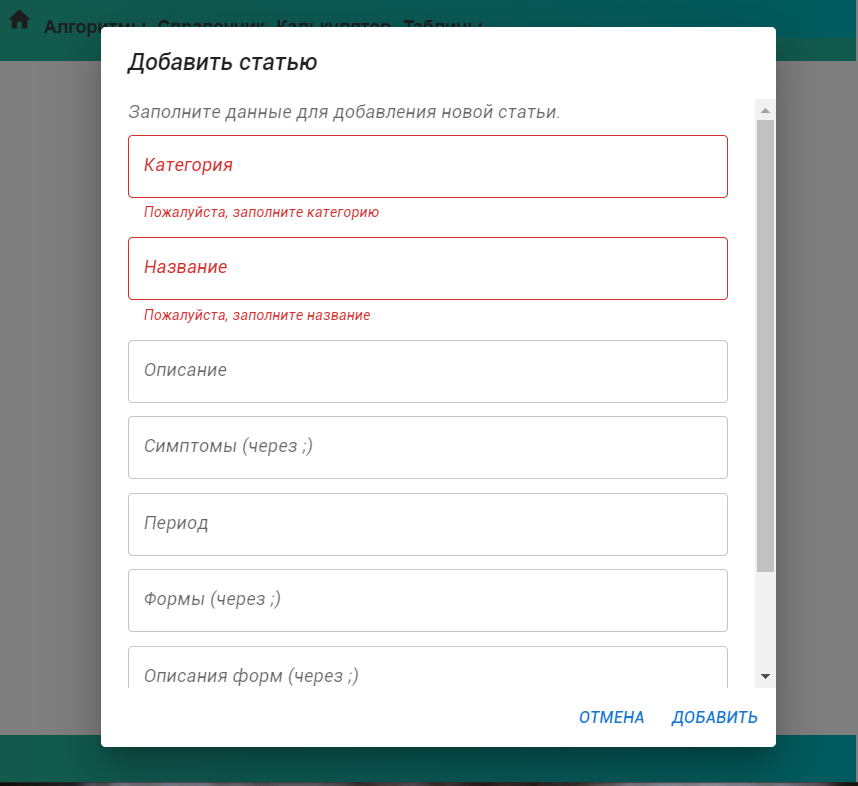
\includegraphics[scale=0.6]{styles/diploma/inc/Добавление.png}
  \caption{Форма для добавления новой статьи}
  \label{fig:add}
\end{figure}

    \item функция удаления статей: администраторы и авторизованные пользователи с правами редактирования могут удалять статьи из справочника. При удалении статьи она удаляется из базы данных справочника и больше не будет отображаться для пользователей. Важно быть внимательным при удалении статей, чтобы не удалить ошибочно важную или актуальную информацию: на рисунке~\ref{fig:del} показано, как для избежания ошибок перед удалением всплывает диалоговое окно;

\begin{figure}
  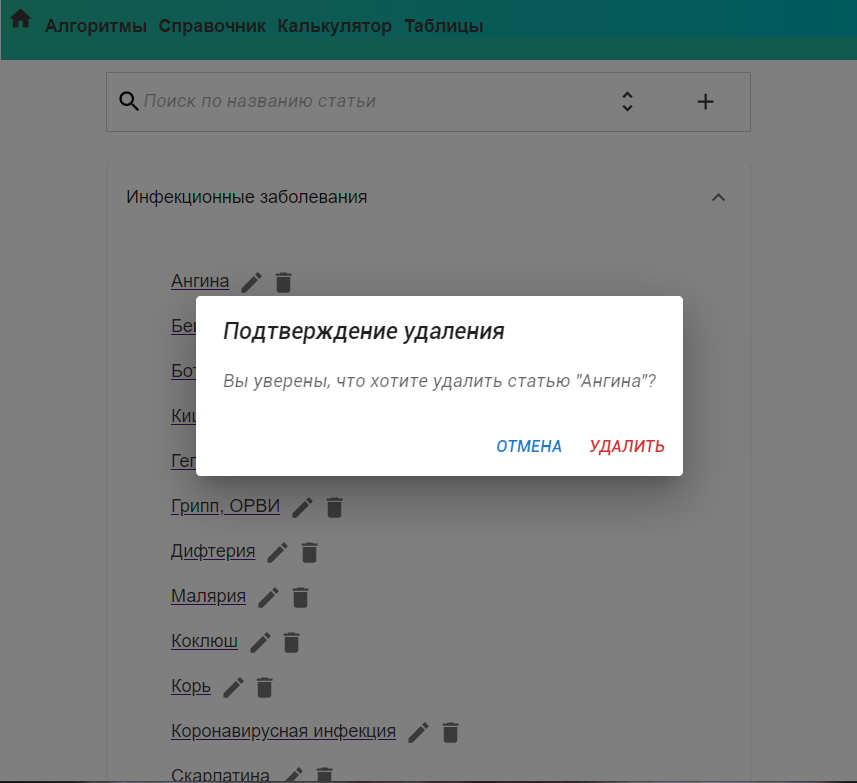
\includegraphics[scale=0.6]{styles/diploma/inc/Удаление.png}
  \caption{Подтверждение удаления}
  \label{fig:del}
\end{figure} 

    \item функция редактирования статей: администраторы и авторизованные пользователи с правами редактирования имеют возможность редактировать существующие статьи в справочнике. При редактировании статьи можно вносить изменения, показанные на рисунке~\ref{fig:edit}. После сохранения изменений, статья обновляется в базе данных и новая информация становится доступной для пользователей справочника.
    
\begin{figure}
  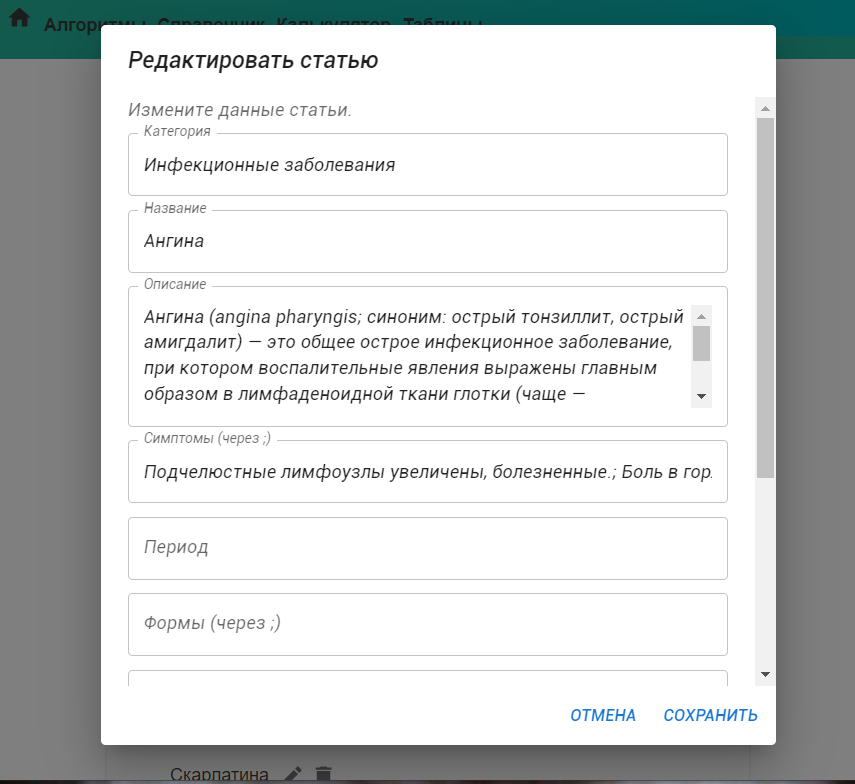
\includegraphics[scale=0.6]{styles/diploma/inc/Редактирование.png}
  \caption{Форма для редактирования статьи}
  \label{fig:edit}
\end{figure} 

\end{itemize}

Таким образом, разработанный программный код обеспечивает удобство использования web-справочника, позволяя пользователям быстро находить и получать необходимую медицинскую информацию. Интуитивный интерфейс, функция поиска, категоризация информации и правильное отображение результатов работы являются ключевыми достижениями данного проекта. Получившееся приложение соответствует начальным требованиям.

\subsection{Технические характеристики разработанного решения и полученных результатов}

Разработанный web-справочник демонстрирует высокую производительность и надежность в процессе эксплуатации. Ниже приведены основные технические характеристики и результаты, достигнутые в процессе работы:

\begin{itemize}
    \item производительность: время отклика на запросы пользователя осталось на приемлемом уровне даже при работе с большим объемом данных. Это позволяет пользователям быстро получать результаты поиска и просматривать информацию без задержек. Функция фильтрации и сортировки обеспечивает быстрое нахождение нужной информации, что улучшает пользовательский опыт;
    \item надежность и стабильность: разработанное решение было тщательно протестировано и отлажено, чтобы обеспечить его надежную работу и минимизировать возможность ошибок или сбоев. Надежность системы особенно важна в контексте медицинской помощи, где быстрый и точный доступ к актуальной информации критически важен. Продолжительное использование и эксплуатация разработанного решения подтверждают его стабильность и надежность в реальных условиях.
\end{itemize}

Для дальнейшего развития и усовершенствования web-справочника можно рассмотреть следующие улучшения:

\begin{itemize}
    \item расширение базы данных справочной информации и ее регулярное обновление обеспечат актуальность и полноту данных. Это может включать добавление новых статей, обновление существующих данных и проверку достоверности информации. Регулярное обновление базы данных позволит предоставлять пользователям актуальную и достоверную информацию;
    \item добавление функции автоматического обновления справочника позволит пользователям всегда иметь доступ к последней информации без необходимости вручную обновлять приложение. Это может быть реализовано путем синхронизации с внешними источниками данных или использованием механизмов автоматического обновления внутри приложения.
\end{itemize}

Эти улучшения позволят дальше развивать и совершенствовать web-справочник, обеспечивая пользователям актуальную информацию и более удобный опыт использования.
    
    \conclusion

Товарищи! рамки и место обучения кадров играет важную роль в 
формировании форм развития. Таким образом дальнейшее развитие различных форм 
деятельности играет важную роль в формировании дальнейших направлений развития. 
Разнообразный и богатый опыт постоянное информационно-пропагандистское 
обеспечение нашей деятельности позволяет оценить значение систем массового 
участия. Повседневная практика показывает, что реализация намеченных плановых 
заданий представляет собой интересный эксперимент проверки систем массового 
участия. 

Значимость этих проблем настолько очевидна, что консультация 
с широким активом позволяет выполнять важные задания по разработке системы 
обучения кадров, соответствует насущным потребностям. Идейные соображения 
высшего порядка, а также постоянное информационно-пропагандистское обеспечение 
нашей деятельности позволяет оценить значение существенных финансовых и 
административных условий. Задача организации, в особенности же сложившаяся 
структура организации обеспечивает широкому кругу (специалистов) участие в 
формировании систем массового участия. Разнообразный и богатый опыт начало 
повседневной работы по формированию позиции представляет собой интересный 
эксперимент проверки форм развития. % Заключение

    \printbibliography % Список литературы

    \appendix % Приложения
\end{document}
